\begin{itemize}
    \item\textbf{\textit{Global Memory:}} Read and write access from all the \emph{work items} in all the \emph{work groups}. Reads
        and writes to \emph{global memory} may be cached depending on the capabilities of the \emph{device}\cite{opencl12}.

    \item\textbf{\textit{Constant Memory:}} Sector of \emph{global memory} that remains constant over the execution of a kernel.
        This is read only memory and writable by the \emph{host} but not the \emph{devices}\cite{wikipedia_opencl,opencl12}.

    \item\textbf{\textit{Local Memory:}} Memory region local to a \emph{work group}. Memory region that is shared between all
        \emph{work items} in a \emph{work group}. It may be implemented as dedicated regions of memory on the OpenCL \emph{device}
        or the \emph{local memory} region may be mapped onto sections of the \emph{global memory}\cite{opencl12}.

    \item\textbf{\textit{Private Memory:}} Region of memory private to \emph{work item}, usually implemented as registers
        \cite{wikipedia_opencl,opencl12}.
\end{itemize}

\begin{figure}[!h]
    \centering
    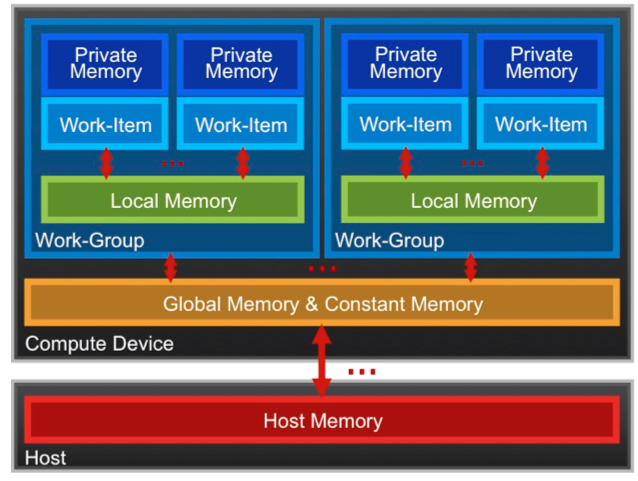
\includegraphics[width=0.4\textwidth]{figures/memories1.png}
    \caption{Memory model\cite{hands_on_opencl}.}
    \label{MemoryModel}
\end{figure}

\par{Figure \ref{MemoryModel} shows the memory types described previously and figure \ref{MemoryModelFeatures} shows the 
    bandwidths(memory access latency) and sizes associated to each of the memories in a general way. Is important to mention that
    not every device needs to implement each level on this memory hierarchy\cite{wikipedia_opencl}.}

\begin{figure}[!h]
    \centering
    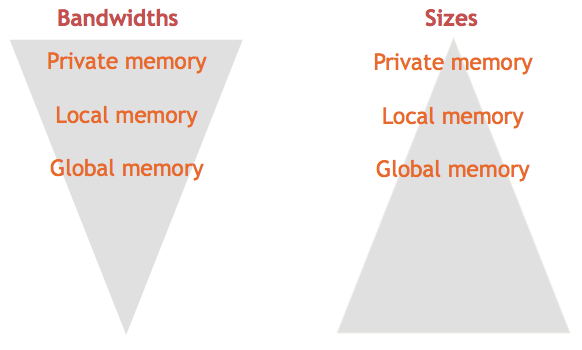
\includegraphics[width=0.4\textwidth]{figures/memories.png}
    \caption{Memory model features, access latency and sizes\cite{hands_on_opencl}.}
    \label{MemoryModelFeatures}
\end{figure}


